\documentclass{article}
\usepackage{graphicx} % Required for inserting images
\usepackage[top=0.9in, bottom=1in, left=1.5in, right=1.5in]{geometry}
\usepackage[utf8]{inputenc}
\usepackage[icelandic]{babel}
\usepackage[T1]{fontenc}
\usepackage[sc]{mathpazo}
\usepackage[parfill]{parskip}
% Tables and lists
\usepackage{booktabs,tabularx}
\usepackage{multirow}
\usepackage{enumerate}
\usepackage{adjustbox}
\usepackage{multicol}
\usepackage{xcolor}
\usepackage{algpseudocode}
\usepackage{tikz}
\usetikzlibrary{arrows, positioning, calc}

% Math
\usepackage{amsmath, amsfonts, amssymb, amsthm}
% Graphics

\usepackage{graphicx}
\usepackage{tikz}
% Code environment
\usepackage{minted}
%\usepackage{bm}
%\usepackage{siunitx}
%\usepackage{animate}
%\usepackage{hyperref}
%\usepackage{movie15}
%\usepackage{multicol}
%\usepackage{changepage}
\title{Gagnasafnsfræði Heimaverkefni 2}
\author{Ragnar Björn Ingvarsson, rbi3}


\begin{document}
	
	\maketitle
	
	\section{}
	\begin{itemize}
		\item[a)] \textbf{Accounts:} \textit{acctNo},
			\textit{type},
			\textit{balance}

		\textbf{Customers:} \textit{firstName},
			\textit{lastName},
			\textit{idNo},
			\textit{account}
		\item[b)] \textbf{Accounts:}

			(12345, sparisjóðsreikningur, 13000), 

			(23456, hlaupareikningur, 2000), 

			(34567, hlaupareikningur, 250)

			\textbf{Customers:}

			(Jón, Sigurðsson, 901-222, 12345),

			(Sigríður, Jónsdóttir, 805-333, 34567),

			(Línus, Gauti, 805-333, 23456)

		\item[f)] \textit{acctNo:} CHAR(5) ef engir reikningar
			munu eiga sér stað með númerið en INT ef svo er.

		\textit{type:} VARCHAR(30) 30 ætti að vera nóg fyrir 
		allar týpur reikninga.

		\textit{balance:} INT

		\textit{firstName:} VARCHAR(50) 50 til að gera ráð fyrir 
		flestum mögulegum nöfnum.

		\textit{lastName:} VARCHAR(50) eins hér.

		\textit{idNo:} CHAR(7) char hér þar sem lengd virðist ekki 
		eiga að vera breytileg.

		\textit{account:} CHAR(5) eins hér og með \textit{acctNo} 
		þar sem ef reikningar eru notaðir þá er betra að hafa INT
	\end{itemize}

	\newpage
	\section{}

	\begin{itemize}
		\item[a)]
	\begin{verbatim}
SELECT address
FROM MovieStar
WHERE name LIKE 'Alec Baldwin';

Baldwin Av.
	\end{verbatim}

		\item[b)]
	\begin{verbatim}
SELECT address
FROM MovieStar
WHERE name LIKE 'Harrison Ford';

Prefect Rd.
	\end{verbatim}

		\item[c)]
	\begin{verbatim}
SELECT starName
FROM StarsIn
WHERE movieTitle LIKE '%Star%' OR movieYear < 1940;

Carrie Fisher
Mark Hamill
Harrison Ford
	\end{verbatim}
	
		\item[d)]
	\begin{verbatim}
SELECT name
FROM MovieExec
WHERE netWorth < 50000000;

Calvin Coolidge
	\end{verbatim}
	\end{itemize}	

	\begin{center}
	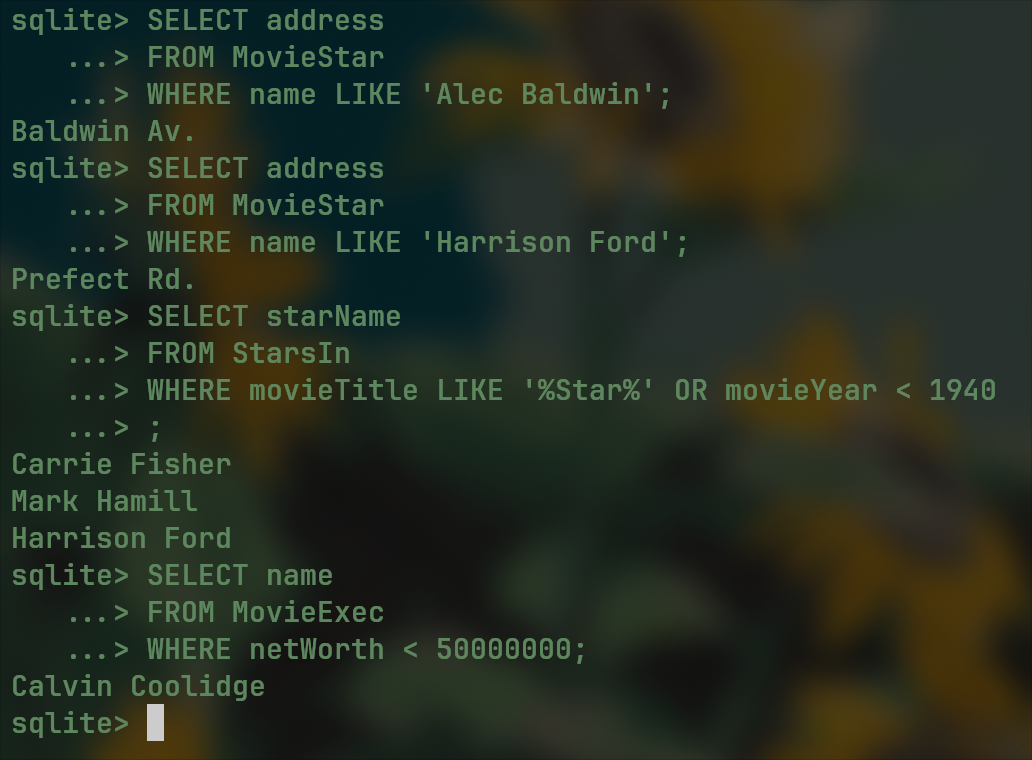
\includegraphics[scale=0.375]{data.png}
	\end{center}


\end{document} 
